\documentclass[main.tex]{subfiles}

\begin{document}

\section*{Goal}
Last chapter, we took steps to ensure that friction was minimized by using the dynamics track and cart. This time we want to study the influence of frictional forces on our system. We will do this by substituting the dynamics track and cart for a plank of wood and a wooden block respectively.

\section*{Equipment}
\begin{itemize}
\item
PASCO Capstone Software
\item
850 Universal Interface (850UI)
\item
Wooden board, wood block with felt attached
\item
Support rod
\item
Meter stick
\item
Mass hanger and masses
\item
Photogate Pulley
\item
String
\item
Triple-beam balance
\end{itemize}•

\section*{Theory}


\subsection*{Static Friction}

\begin{wrapfigure}{r}{0.5\textwidth}
\centering
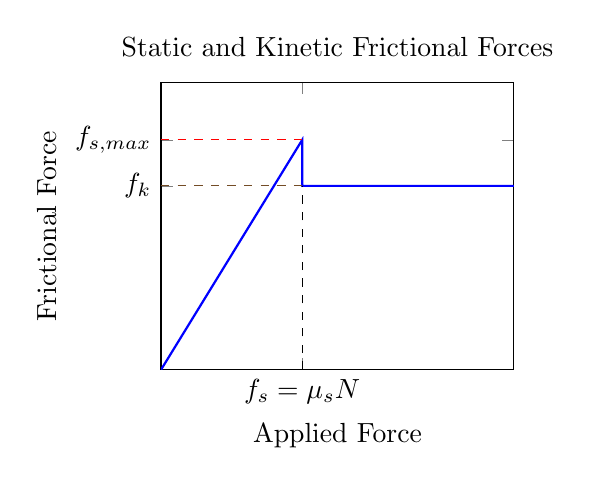
\begin{tikzpicture}
\begin{axis}[
	title={Static and Kinetic Frictional Forces},
	xlabel={Applied Force}, ylabel={Frictional Force},
	xtick={2}, ytick={1.6,2},
	xticklabels={$f_s=\mu_s N$}, yticklabels={$f_k$,$f_{s,max}$},
	xmin=0, xmax=5,
	ymin=0, ymax=2.5,
	no markers,
	width=0.5\textwidth
]

\addplot+ [sharp plot,style=thick] coordinates {
	(0,0)
	(2,2)
	(2,1.6)
	(5,1.6)
};
\addplot+ [style=dashed]  coordinates {
	(0,2)
	(2,2)
};
\addplot+ [style=dashed]  coordinates {
	(0,1.6)
	(2,1.6)
};
\addplot+ [style=dashed]  coordinates {
	(2,0)
	(2,1.6)
};

%\draw [decoration={brace,mirror,raise=5pt},decorate]
%	(axis cs:0,0) -- node [below] {$f_s<\mu_s N$} (axis cs:1,0);

\end{axis}
\end{tikzpicture}
\caption{}\label{fig:FrictGraph}
\end{wrapfigure}

Imagine we are trying to move a box across the floor. When we initially apply a force to the box it may not move because the \emph{static frictional force} that the floor applies to the box is equal and opposite to our applied force. In order to move the box, we will need to overcome this static frictional force. As we increase the applied force on the box, the static frictional force, $\boldsymbol{f}_s,$ will increase roughly linearly as seen in Figure~\ref{fig:FrictGraph}. The static frictional force is defined by the relation,
\begin{equation}
f_s\leq\mu_s N,
\end{equation}
where $f_s$ and $N$ are the magnitudes of the static frictional force and the normal force and $\mu_s$ is called the \emph{coefficient of static friction}.

\begin{wrapfigure}{r}{0.5\textwidth}
\centering
\begin{tikzpicture}[
	m/.style={rectangle,draw=black,fill=brown,minimum size=0.5cm,thin},
	force/.style={>=latex,draw=blue,fill=blue,thick}
]

\begin{scope}[rotate=25]
	\node[m,transform shape] (m) {$M$};
	\coordinate (origin) at (-1.5,-0.5); \coordinate (PlankEnd) at (1.5,-0.5); 
	\coordinate (projend) at ($ (origin) + (1.5,{sin(-44)}) $); \coordinate (End) at ($(origin)!(PlankEnd)!(projend)$);
	\draw[fill=lightgray] (-1.5,-0.25) rectangle (1.5,-0.5);

	\draw[force,->] (m.center) -- ++(0,1) node [above] {$N$};
	\draw[force,->] (m.west) -- ++ (-1,0) node [left] {$F_{applied}$};
	\draw[force,->] (m.east) -- ++(1,0) node [right] {$f_s$};
\end{scope}
	\draw[force,->] (m.center) -- ++(0,-1) node [right,yshift=3pt] {$Mg$};

	\draw[thick] (origin) -- node [midway,yshift=-6pt] {Length} (End) -- node [midway,sloped,yshift=6pt] {Height} (PlankEnd);

	\tikzAngleOfLine(origin)(PlankEnd){\AngleStart}
	\tikzAngleOfLine(origin)(End){\AngleEnd}

	\draw (origin)+(\AngleStart:0.5cm) arc (\AngleStart:\AngleEnd:0.5cm);
	\node [right,yshift=1pt] at ($(origin)+({(\AngleStart+\AngleEnd)/2}:0.5cm)$) {$\theta$};

\end{tikzpicture}
\caption{} \label{fig:StatFriction}
\end{wrapfigure}

In our experiment we will experimentally determine $\mu_s$ of our two materials on our object. Here we will use an inclined plane as shown in Figure~\ref{fig:StatFriction}. To determine $\mu_s$ we want to set $\theta$ so that our object is on the verge of moving. At this point, $f_s=f_{s,max}=\mu_s N.$ If we analyze our setup we can write the system of equations,

\begin{subequations}
\begin{align}
\sum F_x &=F_{app}-f_s=0 \\
\sum F_y &=N-mg\cos\theta=0.
\end{align}•
\end{subequations}•
With some careful manipulation of the above system of equations we find that the coefficient of static friction can be found as,
\begin{equation}\label{eq:mus}
\mu_s=\tan\theta=\frac{Height}{Length},
\end{equation}
where $Height$ and $Length$ are as defined on Figure~\ref{fig:StatFriction}.

\subsection*{Kinetic Friction}
In our kinetic friction experiment we will use the same setup as in Chapter~\ref{chap:Force}, but with one important difference. Whereas in Chapter~\ref{chap:Force} we used the dynamics track and cart to minimize friction, this time we will use a block of wood against a plank of wood to generate a noticeable frictional force.

\begin{wrapfigure}{r}{0.5\textwidth}
\centering
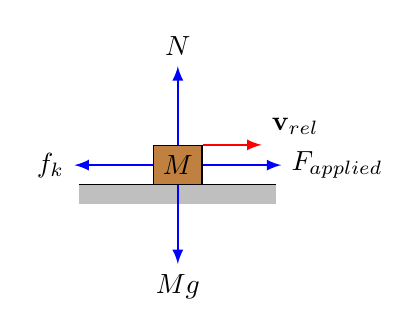
\begin{tikzpicture}[
	m/.style={rectangle,draw=black,fill=brown,minimum size=0.5cm,thin},
	force/.style={>=latex,draw=blue,fill=blue,thick},
	velocity/.style={>=latex,draw=red,fill=red,thick}
]

	\node[m] (m) {$M$};
	\fill[lightgray] (-1.25,-0.25) rectangle (1.25,-0.5);
	\draw (-1.25,-0.25) -- (1.25,-0.25);

	\draw[force,->] (m.north) -- ++(0,1) node [above] {$N$};
	\draw[force,->] (m.east) -- ++ (1,0) node [right] {$F_{applied}$};
	\draw[force,->] (m.south) -- ++(0,-1) node [below] {$Mg$};
	\draw[force,->] (m.west) -- ++(-1,0) node [left] {$f_k$};

	\draw[velocity,->] (m.north east) -- ++(0.75,0) node [above right] {$\mathbf{v}_{rel}$};

\end{tikzpicture}
\caption{} \label{fig:KinFriction}
\end{wrapfigure}
The kinetic frictional force $\boldsymbol{f}_k$ describes a force that opposes the velocity of the body relative to its frictional substrate. In common cases, the relative velocity $\mathbf{v}_{rel}$ is generated by an applied force, so $F_{applied}$ and $\mathbf{v}_{rel}$ point in the same direction, as in Figure~\ref{fig:KinFriction}. The kinetic frictional force can be experimentally found to be be approximately proportional to the \emph{magnitude} of of the normal force by the relation,
\begin{equation} \label{eq:KinFriction}
f_k=\mu_kN,
\end{equation}
where $\mu_k$ is a constant called the \emph{coefficient of kinetic friction}. In reality Equation~\eqref{eq:KinFriction} is only an approximation because $\mu_k$ might depend on the velocity of the object relative to the surface.  For the purposes of our experiment however we will consider that $\mu_k$ \emph{is dependent primarily on the materials involved} and possibly on a few other variables that we will check in today's experiment.

As in Chapter~\ref{chap:Force}, we consider a mass $M$ moving on a horizontal surface and pulled into motion by the weight of a vertically hanging mass $m.$ If we set up our force diagram as we did last time we can get the system of equations,
\begin{subequations}
\begin{align}
M: 	\sum F_x &= T-f_k=Ma\\
	\sum F_y &=N-Mg=0\\
m:	\sum F_x &=0\\
	\sum	F_y &=T-mg=-ma,
\end{align}
\end{subequations}
which we can, with some work, find an expression for the coefficient of kinetic friction as,
\begin{equation} \label{eq:muk}
\mu_k=\frac{mg-(M+m)a}{Mg}.
\end{equation}•

\section{Setup I: Static Friction}
In this setup we will slowly increase the inclination of our board until we reach the critical point where our block is on the verge of sliding down the board. We will then use the measurements to calculate the coefficient of static friction of the different materials on the block.

\subsection*{Procedure}
\begin{enumerate}
\item \label{step:StatFrictStart}
Set the support rod up so that the crossbar is as low as possible.
\item
Place one end of the board on the support rod crossbar and the other end on table.
\item
Place the block so its largest smooth surface is on the board.
\item
Raise the height of the board by 1 cm until the block just starts to slide.
\item\label{step:StatFrictEnd}
Measure and record the height and length as shown in Figure~\ref{fig:StatFriction} into the data table.
\item
Repeat steps~\ref{step:StatFrictStart}--\ref{step:StatFrictEnd} for the small smooth side, and both large and small rough sides of the block.
\end{enumerate}

\subsection*{Analysis}
\begin{enumerate}
\item 
Using the lengths found earlier calculate the coefficients of static friction of each side of the block using Equation~\eqref{eq:mus}.
\item
Average the coefficients of the smallest and largest smooth sides together.
\item
Average the coefficients of the smallest and largest rough sides together.
\end{enumerate}•

\begin{question}
Why is the equation for the coefficient of static friction independent of the weight of the block?
\end{question}

\section{Setup II: Kinetic Friction}
For this setup, the Photogate Pulley will measure the motion of the block sliding on a horizontal surface. The block is connected by a string to a hanging mass, We will vary the mass, surface area of the block, the type of material between the block and the surface, and the amount of hanging mass to change the circumstances of the block. Capstone will then record and display the data by plotting the speed vs time, the slope of which will be the average acceleration of the block for each trial.
\begin{enumerate}
\item
Start Capstone.
\item
Mount the Photogate Pulley at the edge of the board and table top as shown.

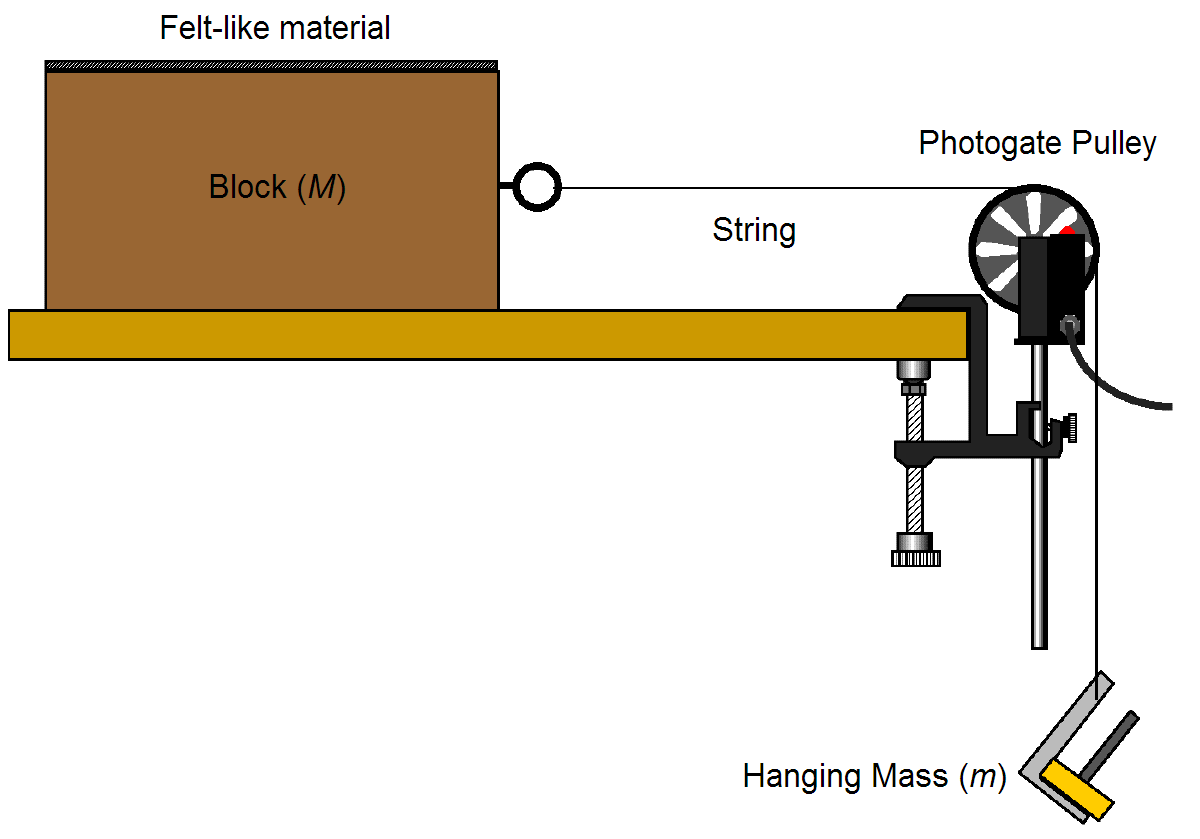
\includegraphics[width=\textwidth]{Friction_Setup}

\item
Attach the Photogate Pulley to the 850UI.
\item
Under ``Hardware Setup" connect the ``Photogate with Pulley" in the appropriate port. Click ``Hardware Setup" to hide it.
\item
Double-click ``Graph" in the toolbar on the right.
\item
For the vertical axis choose ``Linear Speed (m/s)."
\end{enumerate}•

\subsection*{Procedure}
\begin{enumerate}
\item
Measure and record the mass of the block of wood ($M$).
\item
Use a piece of string that is about 10 cm longer than the distance from the top of the board to the floor. Attach one end to the string to the block. Attach the mass hanger to the other end of the string.
\item \label{step:LargeSmooth}
Run \#1 \& \#2---Large, Smooth Surface
\begin{enumerate}
\item 
Place the block so its largest smooth surface is on the horizontal surface.
\item
Put enough mass on the the mass hanger so that the block will slide on the surface without needing an initial push. Measure and record the value of the total hanging mass ($m$).
\item\label{step:LargeSmooth_start}
Pull the block away from the Photogate Pulley until the hanging mass is almost up to the pulley. Hold the block in place. Turn the pulley so the Photogate's beam is not blocked. (The LED on the Photogate will be off when the beam is clear.)
\item \label{step:LargeSmooth_end}
Click on the Record button and release the block. Click on the Stop button to end data collection just before the block hits the pulley. Stop the block so that it does not hit the Photogate Pulley.
\item
Repeat steps~\ref{step:LargeSmooth_start}--\ref{step:LargeSmooth_end}.
\end{enumerate}
\item
Run \#3---Different Mass of Block
\begin{enumerate}
\item
Double the mass of the block by placing a mass approximately equal to that of the block on top of the block.
\item
Measure and record the total mass of the block system ($M$).
\item
Double the hanging mass. Measure and record the total hanging mass ($m$).
\item
Repeat steps~\ref{step:LargeSmooth_start}--\ref{step:LargeSmooth_end}.
\end{enumerate}•
\item
Run \#4---Different Surface Area
\begin{enumerate}
\item
Remove the extra mass from the block.
\item
Place the block so that its smallest smooth side is on the horizontal surface. Adjust the height of the Photogate Pulley so that the string remains level with the horizontal surface.
\item
Use the same hanging mass we used in step~\ref{step:LargeSmooth} (\emph{not} Run \#3) so we can compare the runs.
\item
Repeat steps~\ref{step:LargeSmooth_start}--\ref{step:LargeSmooth_end}.
\end{enumerate}•
\item
Runs \#5--\#7---Different Hanging Mass
\begin{enumerate}
\item
Return the block so the largest smooth side is on the horizontal surface.
\item
Put an amount of mass on the hanger that is larger than the amount we used in step~\ref{step:LargeSmooth}. Measure and record the total hanging mass ($m$).
\item
Repeat steps~\ref{step:LargeSmooth_start}--\ref{step:LargeSmooth_end}.
\item
Repeat the process using two larger hanging masses each larger than the previous. Measure and record the total hanging mass ($m$) each time.
\end{enumerate}•
\item
Runs \#8 \& \#9---Different Surface Material 
\begin{enumerate}
\item
Place the block so that its largest rough side is on the horizontal surface.
\item
Put enough mass on the mass hanger so that the block will slide on the surface without needing an initial push. Measure and record the value of the total hanging mass ($m$).
\item
Repeat steps~\ref{step:LargeSmooth_start}--\ref{step:LargeSmooth_end} to see how the different material affects the coefficient of kinetic friction.
\item
Place the block so its smallest rough side is on the horizontal surface.
\item
Repeat steps~\ref{step:LargeSmooth_start}--\ref{step:LargeSmooth_end} using the same hanging mass as we did for the largest rough side so we can compare the two runs.
\end{enumerate}•
\end{enumerate}•

\subsection*{Analysis}
\begin{enumerate}
\item \label{step:FrictionAnalysis_start}
Using the Select Data Run button 
\includegraphics{Select_Data_Run} display only Run \#1.
\item
For all data runs we will use a linear fit. The slope of the fit line will be the average acceleration of the block.
\item
If necessary, use the Selection Tool 
\includegraphics{Selection_Tool} to highlight only the relevant portion of the data. 
\item \label{step:FrictionAnalysis_end}
Record the acceleration in the data table.
\item
\textbf{Print} a copy of the graph for all group members.
\item
Repeat steps~\ref{step:FrictionAnalysis_start}--\ref{step:FrictionAnalysis_end} for each of the remaining runs.
\item
Calculate $\mu_k$ for each run using Equation~\eqref{eq:muk}.
%\item
%Calculate and record on the data table for Runs \#1 and \#2 the mean value of $\mu_k,$ and the discrepancy between the two values. We will take this discrepancy as indicating the typical experiment error in all our measurements of $\mu_k.$ (Of course, it may happen to be unusually small or large, but this is the best we can do with our present set of measurements.)
%\item
%Calculate an record all the percent discrepancies of $\mu_k$ relative to $\mu_{k0},$ namely,
%\[
%\left(\frac{\mu_k}{\mu_{k0}-1}\right)100\%.
%\]
\end{enumerate}

\begin{question}
How does the coefficient of kinetic friction vary with the mass of the block? Is this variation significant? %(By ``significant," we mean that \emph{the percent discrepancy is more than twice the percent error.} If our answer is ``No, it is not significant," then we are saying that, within the limits of measurement error, $\mu_k$ can be taken as a constant.
\end{question}
\begin{question}
How does the coefficient of kinetic friction vary with the area of contact between the block and the horizontal surface? Is this variation significant?
\end{question}
\begin{question}
How does the coefficient of kinetic friction vary with the type of material between the block and the horizontal surface? Is this variation significant?
\end{question}
\begin{question}
When we used the different type of material, how does the coefficient of kinetic friction vary with the area of contact between the block and the horizontal surface? Is this variation significant?
\end{question}
\begin{question}
How does the coefficient of kinetic friction vary as the speed varied due to the different hanging masses? Is this variation significant?
\end{question}
\begin{question}
When the mass of the block is increased, does the force of kinetic friction increase? Why?
\end{question}

\begin{samepage}
\hrulefill \\
\emph{Chapter~\ref{chap:Friction}:} \textbf{Static \& Kinetic Friction}
\begin{enumerate}
\item
\textbf{(1)} Title Page
\item
\textbf{(5)} Purpose
\item
\textbf{(16)} Theory for both Static and Kinetic Friction---Should include free-body diagrams.
\item
\textbf{(2)} Data Sheet
\item
\textbf{(6)} Sample Calculations for Kinetic Friction
\item
\textbf{(2)} Graph from Kinetic Friction
\item
\textbf{(14)} Answers to questions.
\item
\textbf{(4)} Conclusion
\end{enumerate}•

\newpage
\begin{doublespace}
\section{Data Sheet}
\subsection*{Static Friction}
\begin{tabular}{lll}
Large Smooth Side: & Height=\rule[-1mm]{2.5cm}{.1pt}m & Coefficient $\mu_s$=\rule[-1mm]{2.5cm}{.1pt}\\
& Length=\rule[-1mm]{2.5cm}{.1pt}m &\\

Small Smooth Side: & Height=\rule[-1mm]{2.5cm}{.1pt}m & Coefficient $\mu_s$=\rule[-1mm]{2.5cm}{.1pt}\\
& Length=\rule[-1mm]{2.5cm}{.1pt}m &\\

Large Rough Side:& Height=\rule[-1mm]{2.5cm}{.1pt}m & Coefficient $\mu_s$=\rule[-1mm]{2.5cm}{.1pt}\\
& Length=\rule[-1mm]{2.5cm}{.1pt}m &\\

Small Rough Side: & Height=\rule[-1mm]{2.5cm}{.1pt}m & Coefficient $\mu_s$=\rule[-1mm]{2.5cm}{.1pt}\\
& Length=\rule[-1mm]{2.5cm}{.1pt}m &\\
\end{tabular}\\

\noindent
Average Smooth Sides Coefficient $\mu_s$=\rule[-1mm]{2.5cm}{.1pt}\\
Average Rough Sides Coefficient $\mu_s$=\rule[-1mm]{2.5cm}{.1pt}

\subsection*{Kinetic Friction}
\begin{tabbing}
Mass of block ($M$):\= \rule[-1mm]{2.5cm}{.1pt}kg (Except Run \#3)\\
\>\rule[-1mm]{2.5cm}{.1pt}kg (Run \#3)
\end{tabbing}

%Run \#1 and \#2 only:\\
%\begin{tabular}{ll}
%Average value of $\mu_k$:& $\mu_{k0}:\rule[-1mm]{2.5cm}{.1pt}$\\
%Percent discrepancy of $\mu_k$:& \%-Error:\rule[-1mm]{2.5cm}{.1pt}
%\end{tabular}\\


\begin{tabular}{|c|c|c|c|}
\hline
Run \# & Hanging Mass $m$ (kg) & Acceleration $a\; (\text{m}/\text{s}^2)$ & Coefficient $\mu_k$\\
\hline
1 &&&\\
\hline
2 &&&\\
\hline
3 &&&\\
\hline
4 &&&\\
\hline
5 &&&\\
\hline
6 &&&\\
\hline
7 &&&\\
\hline
8 &&&\\
\hline
9 &&&\\
\hline
\end{tabular}•
\end{doublespace}

\end{samepage}

\end{document}